\subsection{Clique in graph theory}

\renewcommand{\CURPATH}{MaxSMT/clique}

Graph is a group of nodes, some of them may be connected with each other, some are not.
One of the popular examples is the map of country: there are cities and roads.
"Cities" are called "nodes" or "vertices" in mathematics lingo, while "roads" are called "edges".
Another popular example of graph is computer network, including Internet.
Computer network is graph indeed, but it's closer to "sparse graph", because for the most part, computer networks are trees.

"Clique" in everyday speech (especially in political news) denotes a tight-knit group of people inside of some community.
In graph theory, "clique" is a subgraph (part of graph) each vertices ("nodes" or "members") of which are connected with each other.

\subsubsection{Social graph: simple example}

"Social graph" is a graph representing social links.
Here is example I made in Wolfram Mathematica:

\begin{lstlisting}
community = 
 Graph[{John <-> Mark, John <-> Alice, Mark <-> Alice, Tim <-> Alice, 
   Matthew <-> John, Matthew <-> Mark, Tim <-> John, Drake <-> Tim, 
   Bob <-> Drake, Bill <-> Mark, Bob <-> Alice, Tim <-> Mark}, 
  VertexLabels -> "Name"]
\end{lstlisting}

\begin{figure}[H]
\centering
\frame{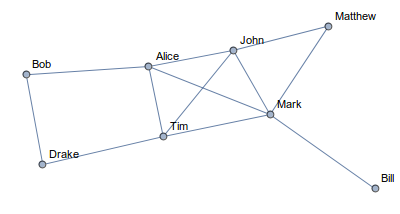
\includegraphics[scale=0.7]{\CURPATH/graph1.png}}
\end{figure}

Let's try to find largest clique:

\begin{lstlisting}
In[]:= clique = FindClique[community]
Out[]= {{John, Mark, Alice, Tim}}
\end{lstlisting}

Indeed, each of these four persons is connected to each among other 3.
Wolfram Mathematica can highlight subgraph in graph:

\begin{lstlisting}
HighlightGraph[community, clique]
\end{lstlisting}

\begin{figure}[H]
\centering
\frame{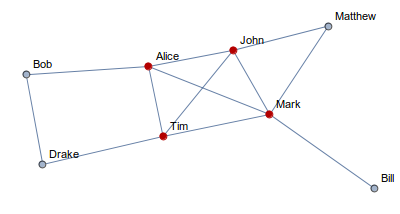
\includegraphics[scale=0.7]{\CURPATH/graph2.png}}
\end{figure}

\subsubsection{Social graph: IRC network}

Internet Relay Chat (IRC) is popular among open-source developers.
One of the most popular IRC networks is Freenode.
And one of the most crowded IRC channel there is \#ubuntu, devoted to Ubuntu Linux.
I used data from it, because all logs are available (starting at 2004), for example:
\url{http://irclogs.ubuntu.com/2015/01/01/%23ubuntu.txt}.

When someone asks, and someone another going to answer the question, IRC users are address each other in this way:

\begin{lstlisting}
[00:11] <synire> How would one find the path of an application installed using terminal?
[00:11] <zykotick9> synire: "whereis foo"
[00:11] <synire> zykotick9: thanks!
\end{lstlisting}

It's not a rule, but well-established practice, so we can recover the information, which users talks to which users most often.
Let's say, we would build a link between two IRC users if 
1) they talk to each other at least 10-11 days (not necessary consequent);
2) do this at least 6 months (not necessary consequent).

The largest cliques of \#ubuntu IRC channel in 10-11 years period are these:

\begin{lstlisting}
* clique size 11
['ubottu', 'ActionParsnip', 'ikonia', 'Ben64', 'zykotick9', 'theadmin', 'dr_willis', 'MonkeyDust', 'usr13', 'bekks', 'iceroot']
* clique size 10
['ubottu', 'ActionParsnip', 'ikonia', 'jrib', 'bazhang', 'Pici', 'iceroot', 'theadmin', 'IdleOne', 'erUSUL']
* clique size 10
['ubottu', 'ActionParsnip', 'ikonia', 'jrib', 'bazhang', 'Pici', 'iceroot', 'theadmin', 'zykotick9', 'usr13']
* clique size 10
['ubottu', 'ActionParsnip', 'ikonia', 'jrib', 'bazhang', 'Pici', 'iceroot', 'sebsebseb', 'IdleOne', 'erUSUL']
* clique size 10
['ubottu', 'ActionParsnip', 'ikonia', 'jrib', 'Dr_Willis', 'Pici', 'edbian', 'IdleOne', 'Jordan_U', 'theadmin']
* clique size 10
['ubottu', 'ActionParsnip', 'ikonia', 'jrib', 'Dr_Willis', 'Pici', 'edbian', 'IdleOne', 'Jordan_U', 'sebsebseb']
* clique size 10
['ubottu', 'ActionParsnip', 'ikonia', 'jrib', 'Dr_Willis', 'Pici', 'erUSUL', 'iceroot', 'IdleOne', 'theadmin']
* clique size 10
['ubottu', 'ActionParsnip', 'ikonia', 'jrib', 'Dr_Willis', 'Pici', 'erUSUL', 'iceroot', 'IdleOne', 'sebsebseb']
* clique size 10
['ubottu', 'ActionParsnip', 'ikonia', 'jrib', 'Dr_Willis', 'Pici', 'erUSUL', 'iceroot', 'ubuntu', 'sebsebseb']
* clique size 10
['ubottu', 'ActionParsnip', 'ikonia', 'Ben64', 'histo', 'bekks', 'MonkeyDust', 'dr_willis', 'iceroot', 'usr13']
...
\end{lstlisting}

% FIXME
Perhaps, these users are frequenters of the channel. List of all cliques are here:
\url{\GitHubBlobMasterURL/\CURPATH/files/IRC/results.txt}.
The output is not terse, because all listed cliques are cliques indeed, and single user or users group can be member of several cliques, that's correct.
Cliques can be overlapped and be members of bigger cliques.
It's possible to produce more human-like results using 
\href{https://en.wikipedia.org/wiki/Community_structure#Algorithms_for_finding_communities}{more complex algorithms for finding communities}.

The source code of my scripts here: \url{\GitHubTreeMasterURL/\CURPATH/files/IRC}.
I used the excellent \href{https://networkx.github.io/}{networkx graph library}.

\subsubsection{Attempt to find communities in IRC social graph}

Wolfram Mathematica can try to find communities within social graph.
Here I will import information about all IRC interactions from the start of 2013 till the summer of 2015.
User nicknames are coded by numbers for simplicity.

\begin{lstlisting}
In[]:= g2 = 
 Graph[{91708 -> 93574, 93414 -> 91525, 93414 -> 89579, 
   90407 -> 93896, 93414 -> 93598, 93809 -> 5909, 93698 -> 93801, 
   93163 -> 83317, 84930 -> 93896, 93414 -> 92947, 93414 -> 91708, 
   93792 -> 92887, 84930 -> 91708, 91708 -> 84930, 88400 -> 93698, 
   ...
   93809 -> 93475, 93698 -> 92887, 93801 -> 93670, 92887 -> 93598}]
\end{lstlisting}

The resulting graph is:

\begin{figure}[H]
\centering
\frame{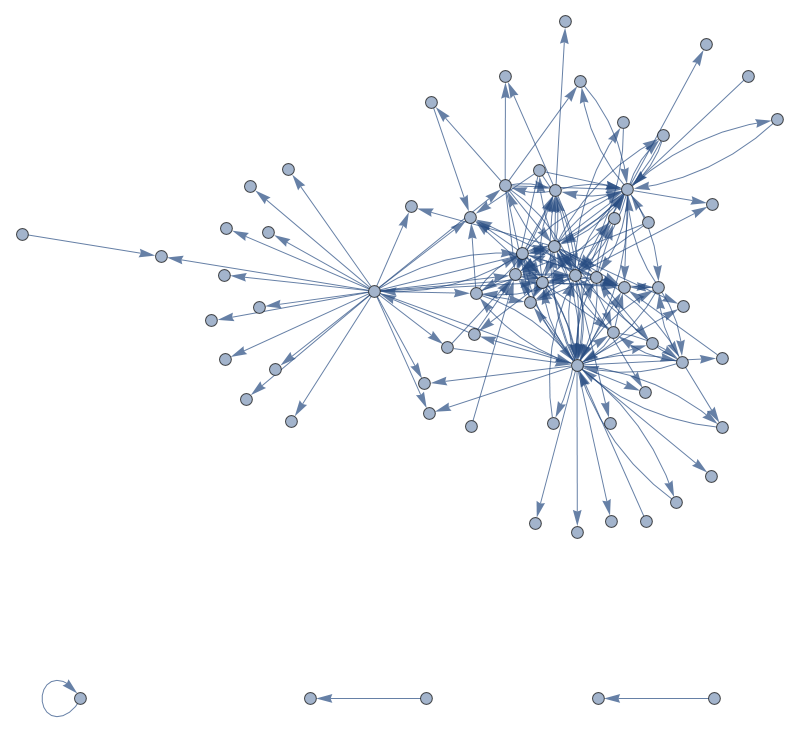
\includegraphics[scale=0.5]{\CURPATH/IRC_g2.png}}
\end{figure}

There some artifacts (at the bottom) which can be ignored so far, I think.
There is prominent centers: one huge and two others are smaller.
I'm not sure, but I can suggest these parts of graph are just users who has different sleep paterns, or, more likely, from different time zones,
so each important time zone (like Americas, Europe, Asia/Oceania) may have their own social communities.
But again, I'm not sure, this should be investigated first.

Let's try to find communities and hightlight them within the graph:

\begin{lstlisting}
c2 = FindGraphCommunities[g2];
HighlightGraph[g2, Map[Subgraph[g2, #] &, c2]]
\end{lstlisting}

\begin{figure}[H]
\centering
\frame{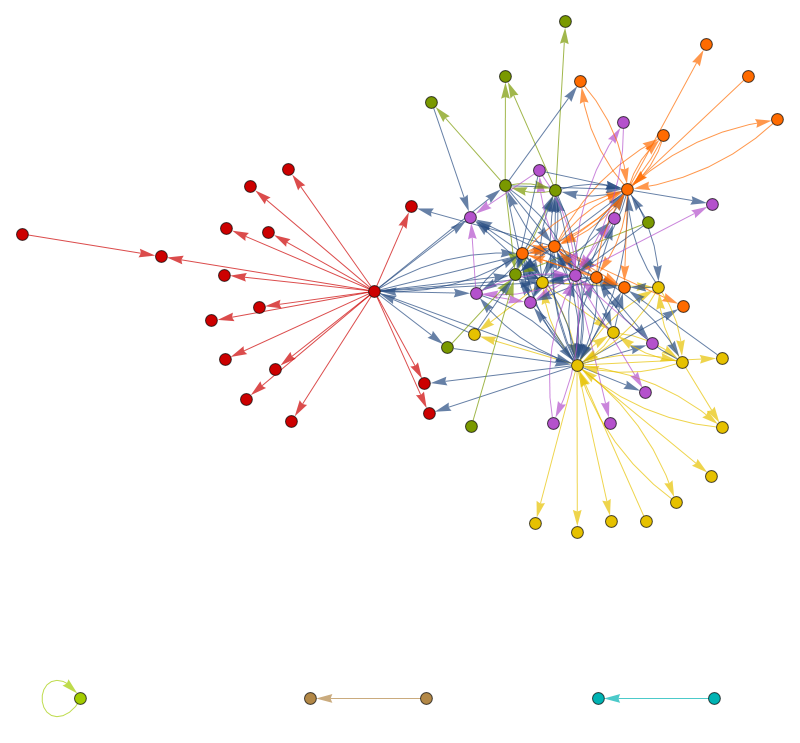
\includegraphics[scale=0.5]{\CURPATH/IRC_c2.png}}
\end{figure}

Hard to say if Mathematica right, but this is what it did.

Now let's take the whole graph of all IRC interactions starting at year 2004 till the summer of 2015.
The graph is much bigger:

\begin{figure}[H]
\centering
\frame{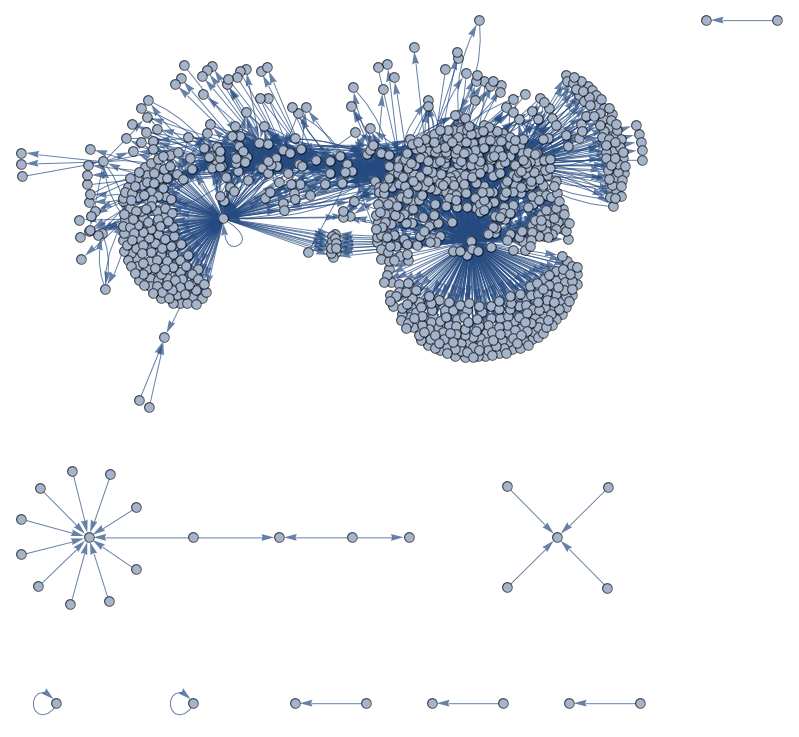
\includegraphics[scale=0.5]{\CURPATH/IRC_g1.png}}
\end{figure}

There are more artifacts.

Let's apply Mathematica's method to find communities:

\begin{figure}[H]
\centering
\frame{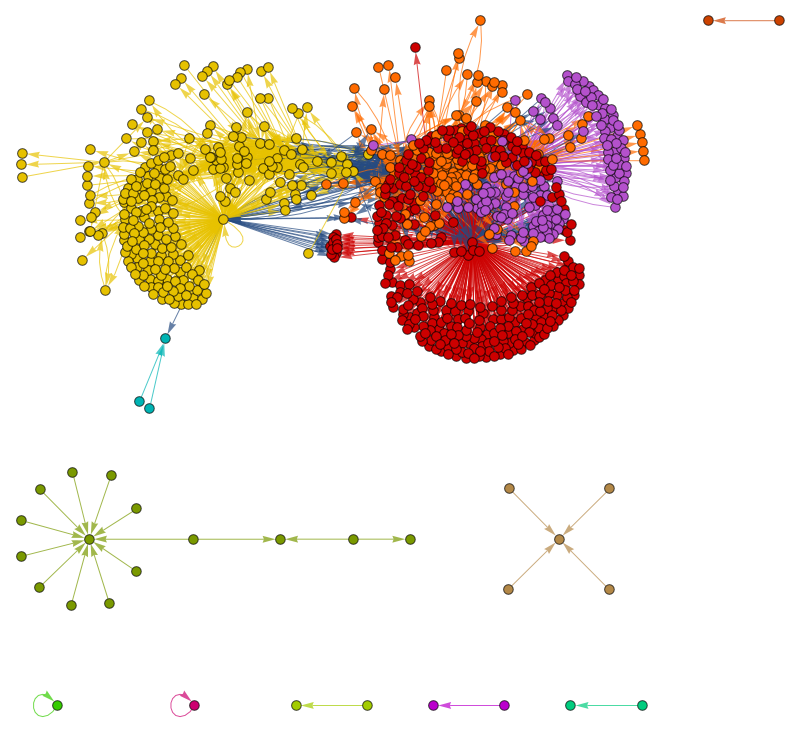
\includegraphics[scale=0.5]{\CURPATH/IRC_c1.png}}
\end{figure}

Is it right? Maybe. Needless to say, since timespan is so long (at least 10 years), we can belive that some communities which may exists in 2004-2006 may be
extinct in 2014-2015 (people got older, lost their interest in Ubuntu Linux, etc), but they all are visible on this graph.

Summary: perhaps, on our next experiment we should filter out IRC data by years and time zones.

\subsubsection{Social graph: social networks}

Perhaps, social networking websites like Facebook and Twitter in the "people you may know" tab shows you users of most populous (by your current friends) cliques.
It may be much more complex in reality, but nevertheless, this is simplest possible way to offer you new social contacts.

\subsubsection{Links graph: Wikipedia}

Wikipedia has a lot of internal links, ~463,000,000 in English Wikipedia as of summer 2015, if not to count user/talk/media pages, etc.
It's possible to build a graph where Wikipedia article is a vertice (or node) and a link from one article to another is edge.
By link between articles we would call the case when the first article has the link to the second article, but also the second has the link to the first one.

Here are some examples of cliques I found this way. Number in parenthesis is clique size.

\begin{itemize}

\item
Chess-related articles (9): Reuben Fine, Mikhail Botvinnik, Samuel Reshevsky, Max Euwe, FIDE, Alexander Alekhine, World Chess Championship, José Raúl Capablanca, AVRO 1938 chess tournament.

\item
Utah-related articles (9): Red Line (TRAX), Utah Transit Authority, Blue Line (TRAX), TRAX (light rail), Salt Lake City, Green Line (TRAX), FrontRunner, University of Utah, Utah.

\item
Articles related to Doctor Who (9): Doctor Who (film), Doctor Who, The Doctor (Doctor Who), Eighth Doctor, The Master (Doctor Who), Gallifrey, TARDIS, Doctor Who Magazine, Seventh Doctor.

\item
Space (9): New Horizons, Pioneer 11, Voyager 1, Europa (moon), Callisto (moon), Ganymede (moon), Jupiter, Io (moon), Pioneer 10.

\item
Hip hop music (9): G-funk, Dr. Dre, Death Row Records, Snoop Dogg, The Chronic, Gangsta rap, West Coast hip hop, N.W.A, Hip hop music.

\item
Metal music (9): Master of Puppets, Thrash metal, Cliff Burton, James Hetfield, Kirk Hammett, Metallica, Kill 'Em All, Ride the Lightning, Dave Mustaine.

\item
The Beatles (8): Break-up of the Beatles, The Beatles, George Harrison, Let It Be, John Lennon, Paul McCartney, Ringo Starr, Abbey Road.

\end{itemize}

Each Wikipedia article within any of these cliques has links to each article in clique.

Full lists of first 1000 largest cliques in English, Russian and Ukrainian Wikipedias plus source code of my scripts is here:
\url{\GitHubTreeMasterURL/\CURPATH/files/wikipedia}.

\subsubsection{Social graph: LiveJournal spammers}

LiveJournal is popular blogging platform in Russian-speaking Internet, which, as any other platform, flooded by spammers.
I once tried, for experiment, to find a way to make distinction between them and human users.
(I did this in 2010-2011, so this information may be not relevant these days).

Aside of false texts spammers posted to their blogs, spammers also mutually friended may spam accounts, so it was not unusual to register, let's say, 1000 fake
accounts and friend each other.

If to build a graph of all links between LiveJournal users, and find largest cliques, there will be prominent unusually large cliques of LiveJournal users, 
up to ~1000.
In real world, you would not easliy find a social group of ~1000 persons who keeps mutual links with each other 
(there is interesting reading about it: \href{https://en.wikipedia.org/w/index.php?title=Dunbar%27s_number}{Dunbar's number}).

Well, spammers could lower this number, so each fake user would have 100-200 mutual friends instead of ~1000 (which is less suspicious), but still, 
cliques were too perfect: each node connected to each other with very low
amount of "external" links, leading to other spammer's cliques and human users.

\subsubsection{Links graph: link farms}

Talking about spammers, there was (or maybe still used today?) also a Black Hat SEO method to build 
"link farms":
this is a collection of many websites which has links to each other.
Interestingly, if you analyze link graph and find cliques, such farms are clearly visible.

